%----------------------------------------------------------------------------------------
%	PACKAGES AND OTHER DOCUMENT CONFIGURATIONS
%----------------------------------------------------------------------------------------
\documentclass[11pt]{report}

\usepackage{lastpage} % Required to determine the last page for the footer
\usepackage{extramarks} % Required for headers and footers
\usepackage{graphicx} % Required to insert images
\usepackage{lipsum} % Used for inserting dummy 'Lorem ipsum' text into the template
\usepackage{hyperref}
\usepackage{float}
\usepackage[bottom]{footmisc}
\usepackage{subcaption}
\usepackage{amsmath}

\linespread{1.1} % Line spacing
\usepackage[total={6in, 8in}]{geometry}

\setlength\parindent{0pt} % Removes all indentation from paragraphs

\begin{document}
\title{Novel Gaming Experiences with Advanced Illumination 
through Augmented Reality: Interim Report}
\author{Terence Tse \\
		Supervisor: Benjamin Glocker\\
		Second Marker: Abhijeet Ghosh}
\maketitle
\newpage
\tableofcontents
\newpage

\section*{Abstract}
Oh
\newpage

\section*{Introduction}
\begin{center}
\textit{I want to create the world.}
\end{center}

Augmented Reality(AR) has come into the limelight once
again with the recent release of the Google Glass. AR has 
been around for a while now, most of the time being
thought of the future of technology but with applications ending up with 
limited use, less than satisfying performance and being gimmicky, it has been
hanging around in the background for a while.
\\ \\
AR in a nutshell is reality, augmented! A view of the real world is presented
to the user but it has been enriched in some sort of way. If you are unaware
of what looking through a Google Glass is like, one pretty well known example 
is the film Terminator. When seeing from Terminator's viewpoint, we are 
presented with a red screen, this is what a normal person would see but in red.
However, on the screen, it has a crosshair, which lock onto a person, their
statistics in the right hand corner, when it's your target, the words flash
in view. This is what augmented reality is.
\\ \\
Of course, we're not all cyborg assassins, hence why things like the Google 
Glass have been created. Our eyes already give us a lot of information about 
the world, but having even more information presented to us than what we
naturally have is Augmented Reality. Already, anyone with a semi-decent mobile
phone can play around and take benefits from Augmented Reality, it does not take
large amounts of processing power to produce an AR image. The key is that AR is
real time, our view gets updated as we see it. 
\\ \\
Augmented Reality is not just limited to some head mounted device. In addition
to our phones, we can use tablets or just plain computers in which to play
with AR. All we need is a camera which can capture the world and then allow 
us to view it either with additional information or even diminished information!
One use case is in the British Maritime museum, where visitors can aim cameras
at special AR exhibits and have the item explained to them visually. The range 
applications of AR are overwhelming, imagine a Dinosaur coming to life in a
History museum and you can see it navigating the halls. Imagine having an
AR mirror that superimposes clothes onto your body that fit, without having
to go and search and try on the clothes themselves. Imagine being on a 
construction project and you are able to view the outcome on your tablet, even
if the old structure has not been cleared away for the new project to begin!
Augmented Reality can do all of that already and the scope of new
applications is, no pun intended, as far as the eye can see!    
\\ \\
As previously stated, AR has many applications in terms of games and 
entertainment. These come in all different styles, from simple use of a camera,
to using fixed feature points as markers, or using patterns as feature points
to identify placement of objects in the scene. Right now, these feature points
are either very simple or immutable. They are something that the computer
can directly identify which is obviously good for performance reasons. However,
what about the ability to create your own feature points on the fly? If we
able to immediately draw feature points and by extraction of these points, 
augment reality based off of these points, it would greatly improve the 
experience of Augmented Reality, removing the need to create the marker 
on a computer and just, for example, grabbing a piece of paper, drawing it
yourself and have it work straight away! I shall refer to this as a feature
drawing throughout the rest of the report. 
\\ \\
However, AR may also be used for more commercial and other practical uses. 
When people think of AR, it usually defaults to thinking about games and 
indeed there is a lot of future in that industry with AR, there are also
Educational uses, Project and Landscape Planning, Commerce and Animation, 
the list goes on. The problem right now is that simple AR applications which
augment a scene with, say a dinosaur or some other object, those generated
images are still quite obviously generated by a computer, especially when 
they try to get more complex. In a bright room, you may place furniture inside
which looks semi-realistic, it has a computed shadow and gradient change. 
However, an ideal situation is when we augment reality and it doesn't even
feel as if anything is different. In other applications, the objects may not
even have an advanced lighting model, solid colours with no depth or 
obscurance may be modelled, thus not even a shadow is created making it 
extremely obvious (whether this is desired or not) to us which objects in
the scene have been artificially generated. It is harder to appreciate this
as an extension of reality when it is so obvious that this object does not
belong in the scene.
\\ \\
This project is focused around these points. First, I'd like to make additions
to the AR realm; I will focus around using Augmented Reality to 
provide not only a novel gaming experience, but also one that can be 
transferred over to more practical use cases while appearing realistic in
addition to have users generate a set of feature points manually in the real scene.
One way that we can drastically improve the realism of a computer generated
image is to improve the illumination model to such a degree that the object
looks like it belongs in the view. 
\\ \\
\subsection*{Project Goals}
The bigger picture and where this project hopes it can contribute and make 
headway into is permitting a dynamic and responsive AR application that allows
creators to quickly draw up environments which can then be visualised. 
Environments can also be changed in real time and will be reflected in the AR
without need for additional user interaction. The completion of this
task will have numerous transferable benefits that were mentioned in the 
SECTION ABOVE. %FILL THIS IN

However, the amount of work that this goal encompasses coul be infintissimal
depending on what kind of features would be deemed necessary, good or just an
extension. There are also numerous parts of a project like this could be 
analysed in much further detail. As a result, the objectives for this project
are:

\begin{itemize}
	\item Create a functioning Augmented Reality program which takes a
		  video stream and overlays a 3D landscape on a contour map created by
		  the user. The contour map may also have other feature points which 
		  indicate other 3D structures to be rendered.
	\item Using a method of video and scene tracking/recognition, allow users
		  to make changes to their contour map and have the landscape update 
		  in real time. This essentially allows dynamically changing 
		  Augmented Reality landscapes.
	\item Perform an analysis on the performance and responsiveness 
		  of the final product of this project. This will be done
		  through user testing.
		 
\end{itemize}

\newpage
\section*{Background}

\subsection*{Augmented Reality}
\begin{center}
What is Augmented Reality(AR) and why should we be interested in it? \\
\end{center}
In recent years, it becomes harder and harder to concisely describe what
constitutes as Augmented Reality. The reason for this being that as technology
improves more and more things are being achieve that allow users to extend
their perceived reality with extra data.\\ 

Simply put, Augmented Reality is when the environment around you can be 
extneded by combining both real and virtual data components. Azuma's 
paper\cite{Azuma97}, \textit{A Survey of Augmented Reality},
describes AR as having the following three characteristics:
\begin{enumerate}
	\item Combines Real and Virtual (data) 
	\item Interactive in real time
	\item Registered in 3D
\end{enumerate}

While these are the basic things that constitute AR, there are three ways, 
outlined in Mackay's paper\cite{Mackay}, \textit{Augmented reality: linking 
real and virtual worlds: a new paradigm for interacting with computers},
in which you can augment reality.\\
These are:
\begin{enumerate}
	\item Augmenting the User
	\item Augmenting Physical devices/objects
	\item Augment the Environment
\end{enumerate}

\underline{Augment the User} \\
Augmenting the user is having the user carrying, wearing or using a device
that provide the user with extra information. When we talk about augmenting
the user, the devices we talk about are usually
heads-up displays (HUDS) which the user will have a screen in front of their
eyes in some shape or form. One example of this is Google Glass, allows
users to project information about what they see or their GPS location onto
parts of the glass. If the user was looking at the Eiffel Tower through their 
glass, with GPS coordinates and a scan of the shape of the Eiffel Tower, 
Google Glass would be able to tell that what the user was looking at. From there,
it can project information about the landmark to the user which would not have
been accessible so easily otherwise! \\

This is one such trivial application of
user worn AR, it is very useful for lesser known things, for example, instead of 
looking at a famous landmark, the user could be an engineer, looking at a 
complex piece of machinery and a HUD allowing them to get information on each
component. This is also being trialled in Medicine, where doctors can use
Augmented Reality to help teach surgical procedures or even help them in
analysis of medical images such as X-Rays.\\

\underline{Augment Devices} \\
When an object or device has a small computer placed into it, it can be 
considered as an augmented device. One example of this is again in 
surgery and medical environments. Having tools such as scalpels or other 
medical equipment fitted with computers to plot out how much of the skin has
to be cut, for example, allows the user to receive much more information
than they would be able to than without. Mackay also talks about these briefly 
in her paper.\\

\underline{Augment the Environment} \\
This form or AR doesn't add any additional hardware to devices nor the user.
It focuses on having external devices, such as projectors or cameras take 
input from the user and use that to transofrm the environment that they are in
or are manipulating. This class of AR is much wider than the two 
aformentionned as there are less things imposed on an object/person which 
allow a larger spectrum of devices to be used. \\

An example of Augmenting the environment is an AR keyboard, a projector displays
a keyboard in front of where it is placed, the user can then "press" keys and
the kyboard will be able to detect which key has been selected and translate it 
into computer input. \\

A more common device is your smart phone! Tablet or even computer screens can
be included in this form of AR. There are plenty of mobile applications that
allow users to experience AR in their own unique way. An example used in the
British Maritime Museum is the ability to take a tablet with predownloaded apps
that allow users to engage in an AR game. Through the game, which is primarily
aimed at children, allows them to learn about the exhibits in a more fun and
interactive way. There are also similar applications in retail, for example
in retail! Augmented reality mirrors are being used to avoid the time in the
changing room and allow customers to "try" on pieces of clothing through
AR by overlaying the garment over their captured video. \\

Another fun implementation of AR is the Augmented Sandbox. A projector and
a camera are used to transform a sandbox into a remoldable landscape. The camera
uses depth sensing and the input from here is transformed into lanscape height
and the projector correspondingly projects land or water onto these areas. The
magic happens when the sand is manipulated and the whole system re-renders the
landscape in real time to provide an interactive augmented environment! Sarah
Reed from the University of California lead the authoring of the persentation
about this piece of tehnology\cite{Reed14}.\\


\subsection*{Computer Vision and Image Processing}
A key part of this project is the Computer Vision aspect. The field of
Computer Vision involves the understanding of data from images and pictures.
"Understanding" is a broad term that encompasses many ways of manipulating or
processing images in order to extract features or points of interest that
can be then used by the computer.

\subsubsection*{Edge Detection}
% Detecting lines and edges of paper, for registration

\begin{center}
	In an image, an edge if a set of pixels that separates to disjoint
	regions.
\end{center}

A key part of Computer Vision is line and edge detection. Edge detection is
the very beginning of how we can start to identify different objects 
within an image. In addition, by stripping an image down to its comprising
edges, we greatly decrease the amount of information in the image whilst
preserving the important parts which we want to operate on. 
As a result, how edges are detected have a large contribution
to what we can do with certain images.  

Edge detection tries to find the set of pixels that separate two 
disjoint areas of an image by analysing sets of neighbouring pixels and 
looking for discontinuities in intensity or texture. A variety of factors
can cause these (local) discontinuities:
\begin{enumerate}
	\item Object colour and texture. If the object has any change in colour or
		  texture, then where the change occurs, an edge will be detected.
	\item A change of surface normal. In the real world, we have 3D objects,
		  as a result, there will be a surface normal change when we consider,
		  say, the top face of a box against the side face. There is an edge
		  between the two and this is partly also due to the next factor.
	\item Illumination. A change of illumination or simply due to some
		  part of the obejct in question casting a shadow will cause some regions
		  of the image to be darker or lighter in intensity, even if said
		  regions are part of the same object. Edges will be detected in this
		  instance.
	\item Two objects. This a large part of why we even do edge detection, to
		  detect objects. If there are two objects, then, likely, there will be
		  a difference in colour and intensities of their constituant pixels.
		  However, this is not always the case and also as can be reasoned from
		  above, these regions may belong to the same multi-coloured object.
\end{enumerate}

When it comes to 

We can distinguish edge detectors into two sets, the Laplacian of Gaussain detectors
and the Gradient-based detectors.

\subsubsection*{Gradient-based detectors}
Gradient edge detectors look for changes of gradient (first-order) of 
neighbouring pixels. Some common gradient-based detectors are Sobel,
Prewitt, Canny and Robert. Each of these detectors starts off with an image
and an x and y kernel. The kernels help determine the gradient change
and y directions of the image, different kernels (size and values) are what
separate the different Gaussian-based detectors. The final gradient magnitude
for a given pixel is then the square root of the sum of these: 

\begin{equation}
	G = \sqrt{\Delta x^2 + \Delta y^2} 
\end{equation}

Users can then set a threshold value for which any pixel with a final
gradient that is above that threshold will be treated and marked as an edge,
the others will be discarded.

\subsubsection*{Laplacian (of Gaussian)-based detectors}
Laplacian based detectors are similar to Gradient-based ones except that 
instead of taking the first derivative, they consider the second derivative.
Their goal is to look for zero-crossings, i.e. local maxima in 
gradient changes (i.e. looking for when gradient starts going negative). The
change of gradient sign, which occurs when second order derivative is 0,
indicates that the intensity of the observed pixels begins changing also. This
method can be coupled with a Gaussian kernel which serves to de-noise the
image by smoothing out the pixel intensities. 


\subsubsection*{Canny Edge Detector}
% Detecting Contours for landscaping

There have been numerous methods of detecting edges put forward,
some Gradient-based and Laplacian based edge detection methods are 
outlined in 
\textit{A Comparison of various Edge Detection Techniques used in Image Processing}
\cite{Shriv12}. However, the most popular edge detector out there is the
Canny Edge detector, put forward by John Canny in his paper
\textit{A Computational Appraoch to Edge Detection}\cite{Canny86}. The paper
dicusses a methematical approach to edge and ridge detection which is then
analysed on in Ding and Goshtasby's paper, 
\textit{On the Canny Edge Detector}\cite{Ding00}. Rashmi's paper,
\textit{Algorithm and Technique on various Edge Detection: A Survey}
\cite{Rashmi13} compares various edge detection algorithms and finds that 
the Canny edge detector comes out on top, with Maini's paper 
\textit{Study and Comparison of Various Image Edge Detection Techniques} 
\cite{Maini} showing the same result.

The Canny Edge detector falls within the Gaussian-based Edge detectors and
can be described algorithmically below:
\begin{itemize}
	\item Apply a Gaussian filter over the image to remove noise by smoothing
	\item Take the Gradient of the image pixels over each direction, just as
		  would be done in a normal Gaussian-based detector.
	\item Apply non-maximum suppression 
		  such that only local maxima are marked as edges (the pixel 
		  has a greater gradient magnitude than all
		  of its neighbours) resulting in a thin edge. The thinning of found
		  edges is to remove some affect of the blur. After this, perform
		  double thresholding, those higher than the threshold are "strong" edges
		  and those under are weak edges.
	\item Another round of removing edges is applied by using hysteresis.
		  This involves identifying "strong" edges,and then removing 
		  all edges that are not connected directly to these strong edges.
\end{itemize}

The steps are more fully explained in the paper by 09gr820, 
\textit{Canny Edge Detection}\cite{09gr820}.

\subsubsection*{Open and Closed contours}
We understand a closed contour to be a loop. By this we mean that if we had
to draw a closed contour, we begin at a point on a piece of paper and end at that
point, either by not removing our pen from the page or, if done so, will resume
at the same point to finish up the contour. The existence of white space between
points on a contour mean that the contour is open, thus not closed. Examples
of open and closed contours can be seen in Figure \ref{fig:closedcontours} and 
Figure \ref{fig:opencontours}.
\\

\begin{figure}[!ht]
	\centering
	\begin{subfigure}[t]{.3\textwidth}
		\centering
		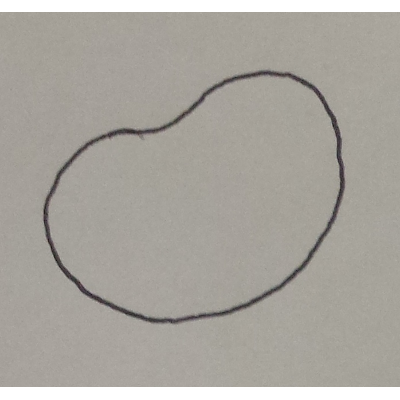
\includegraphics[scale=0.3]{pics/closedloop1.png}
		\caption{Contour is fully closed, no gaps}
	\end{subfigure}
	\hfill
	\begin{subfigure}[t]{.3\textwidth}
		\centering
		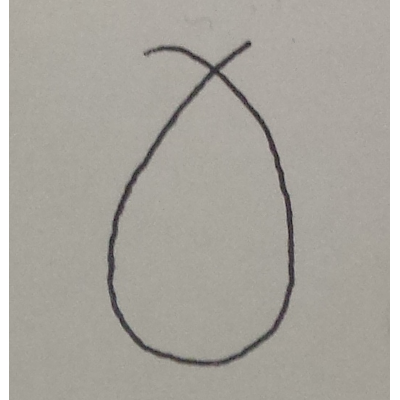
\includegraphics[scale=0.3]{pics/closedloop2.png}
		\caption{Contour is closed, but with artefacts on the ends}
	\end{subfigure}
	\hfill
	\begin{subfigure}[t]{.3\textwidth}
		\centering
		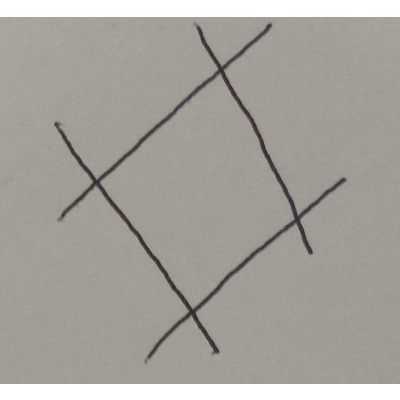
\includegraphics[scale=0.3]{pics/closedloop3.png}
		\caption{This is also a closed contour}
	\end{subfigure}
	\caption{Examples of \textbf{closed} contours}
	\label{fig:closedcontours}
\end{figure}

\begin{figure}[!ht]
	\centering
	\begin{subfigure}[t]{.3\textwidth}
		\centering
		
\includegraphics[scale=0.3]{pics/openloop1.png}
		\caption{A line/edge counts as an open contour}
	\end{subfigure}
	\hfill
	\begin{subfigure}[t]{.3\textwidth}
		\centering
		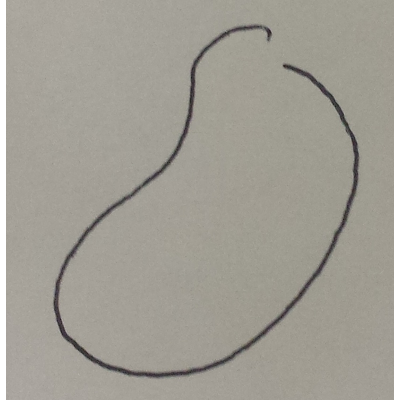
\includegraphics[scale=0.3]{pics/openloop2.png}
		\caption{Contour open as beginning doesn't connect to end}
	\end{subfigure}
	\hfill
	\begin{subfigure}[t]{.3\textwidth}
		\centering
		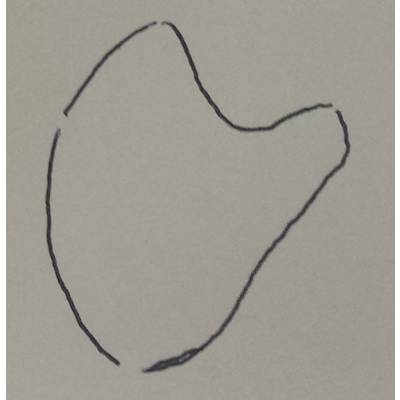
\includegraphics[scale=0.3]{pics/openloop3.png}
		\caption{This contour is open with several gaps}
	\end{subfigure}
	\caption{Examples of \textbf{open} contours}
	\label{fig:opencontours}
\end{figure}

For feature detection, and especially within this project, we look for 
\textit{closed} contours, they provide us with the most information. An open
contour may be linkeed to some kind of feature point but if it is not closed,
its usefulness is very low. In particular, we want closed contours so that any
contours that are drawn within them can then lend themselves to a natural
hierarchy/ordering. In the context of this project, those within closed contours
will represent areas that are of higher elevation than the area contained between
itself and the outer contour. When contours are not closed, it becomes harder
for us to identify this hierarchy and ordering within the image,
which would mean a lot more difficult computation to be done to achieve
our goal of generating a corresponding landscape. Indeed, this is the problem of
many similar projects.

\subsubsection*{Mathematical Morphology}
One technique to help close contours/loops in Computer Vision is \textit{Closing}.
To understand \textit{Closing}, we must first introduce the ideas of 
Mathematical Morphology (MM). MM is a method of analysing geometric objects
and structures, typically used on images but can also be applied to other things
such as graphs. Within MM, there are four basic operators, but for the purpose
of this project, I shall only go into detail about the first three:

\begin{itemize}
	\item Erosion	
	\item Dilation
	\item Closing (Dilation followed by Erosion)
	\item Opening (Erosion followed by Dilation)
\end{itemize}

The operators were originally defined for binary images and so shall be 
described below in that sense, however, the functionality has been extended
to include grayscale images as well, which is very useful when dealing with
photographed images or video feed as will be done within this project.
\\
For these operators, let us assume there is a binary image, with pixels 
holding values of either 0 or 1. In correspondence to a typical colour image,
1 indicates white, a brighter area, of the image and 0 corresponds to a
black pixel. In the erosion and dilation operators, we have this binary
image as input. We also have a corresponding kernel which we will convolute
with the image. This kernel, sometimes referred to as a structuring element,
usually takes the shape of a circle, a 3x3 square or a cross. To achieve
different results from these operators the kernels can be changed, for example
to a 10x10 square hich will cause a more drastic shrink or growth of bright 
areas. For the purpose of explanation, I will assume we are using a 3x3 kernel.

\subsubsection*{Erosion}
\begin{center}
Erosion causes bright areas of images to shrink.
\end{center}

Having the 3x3 kernel anchored at its centre square/pixel, we place align
the kernel with every single pixel on the binary image by superimposing
the kernel's anchor over it. Within the other kernel pixels (a 3x3 neighbourhood
of the pixel in question), we set the pixel under the anchor to the minimum 
value in this neighbourhood. Thus, the only way a pixel can remain white in
a binary image is if it starts off as white and all of its neighbours with 
regard to the kernel shape, are white too. If this is not the case and even 1
is 0 in its neighbourhood, the pixel considered is set to 0. The effect
of this can be seen in Figure \ref{fig:ErosionExample}. As you can see from 
the result, the original shapes have become much thinner and there are now
3 shapes instead of 2. When combined with dilation, it is clear how some contours
can be "opened" as erosion comes as the last step. The result shown in
Figure \ref{fig:ErosionExample} shows how what could be the constituent pixels
of a contour being broken down into 2 separate objects of interest, thus 
\textit{opening} the contour. In addition, erosion can be used to remove
small, likely unimportant, parts of images, such as noise, since any noise
that isn't large enough to be a problem, would be fizzled out by the kernel, 
whose size can be changed to affect noise sensitivity.\\

\begin{figure}[ht]
	\centering
	\begin{subfigure}{.45\textwidth}
		\centering
		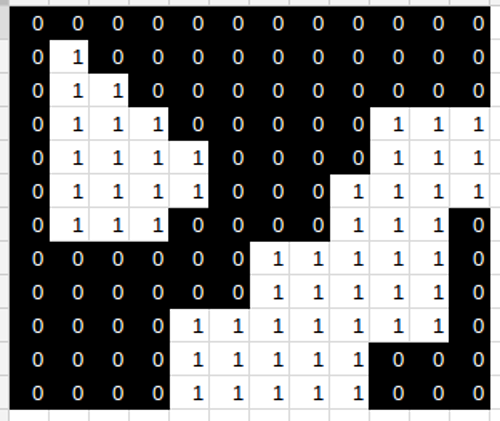
\includegraphics[scale=0.4]{pics/morphologyexample.png}
		\caption{Original Binary Image}
	\end{subfigure}
	\hfill
	\begin{subfigure}{.45\textwidth}
		\centering
		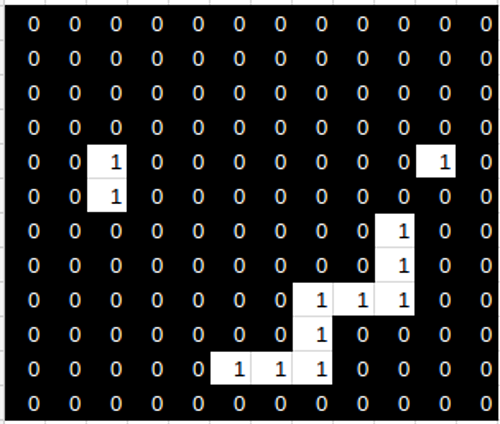
\includegraphics[scale=0.4]{pics/morphologyexample_e.png}
		\caption{Eroded Image}
	\end{subfigure}
	\label{fig:ErosionExample}
	\caption{Erosion}
\end{figure}

\subsubsection*{Dilation}
\begin{center}
	Dilation causes bright areas of image to expand.
\end{center}

Dilation performs the opposite of what erosion would do. We still perform 
convolution with our 3x3 kernel but instead we set the pixel below the
kernel anchor to be the \textit{maximum} value within the 3x3 neighbourhood.
As a result, if there is even a single white pixel in the neighbourhood, the
current pixel will turn white. The only case this will not happen is if the 
pixel started off with a pixel value of 0 and all of its neighbours also had
a value of 0. Figure \ref{fig:DilationExample} shows the result of dilation with
the same original image as shown in the Erosion section above. 
\\
It can be observed from the result above that a dilation greatly increases
the size of the bright area. In addition, if bright areas are suitably close
to one another, it can cause the areas to join into one through the dilation.
This is how contours with small gaps are able to be closed and will aid in the
contour detection process. Again, the kernel size and shape may be changed to
cover a larger area (thus join bright areas further apart) or otherwise 
depending on how sensitive you want the operation to be.

\begin{figure}
	\centering
	\begin{subfigure}{.45\textwidth}
		\centering
		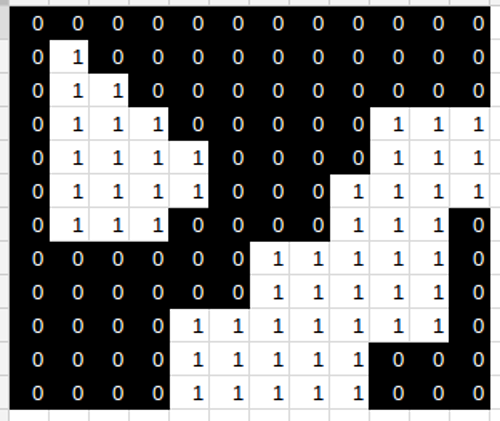
\includegraphics[scale=0.4]{pics/morphologyexample.png}
		\caption{Original Binary Image}
	\end{subfigure}
	\hfill
	\begin{subfigure}{.45\textwidth}
		\centering
		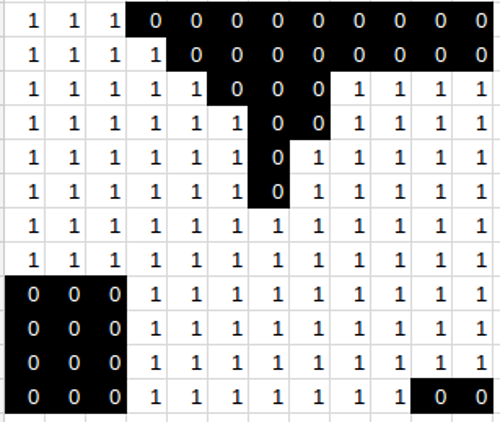
\includegraphics[scale=0.4]{pics/morphologyexample_d.png}
		\caption{Dilated Image}
	\end{subfigure}
	\caption{Dilation}
	\label{fig:DilationExample}
\end{figure}


\subsubsection*{Closing}
\begin{center}
Closing is Dilation followed by Erosion.
\end{center}
Closing is very similar to dilation but it aims to preserve more information.
The Closing operation is no different to erosion or dilation in that we
provide a kernel with which to onvolute the given image with. To perform Closing,
the image first has a dilation operation applied to it with the given kernel. 
After this, erosion is done with the same kernel on this dilated image. \\
By just performing dilation, we do manage to close small gaps in the image, 
however, every pixel is equally distorted by the kernel and so the resulting
image will look quite different to the original shapes, as can be seen
in Figure \ref{fig:DilationExample} above. In order to reduce as much
of this distortion as possible, erosion is used. The overall affect of this is
to make the resulting image be as similar as possible to the outline of the
provided original image. Closing is idempotent, after one pass the resulting
image will not change from further Closings with the same kernel. The effect 
of closing is illustrated in Figure \ref{fig:closing}.\\
The original images starts off with some holes within the image. If we
take this to be a contour discovered by an edge detector, then we can show
how we can close it with \textit{Closing}. After the Dilation stage, the
small holes within the original image have been closed, in addition, the 
boundaries of the bright parts of the picture have been joined due to their
proximity and the kernel shape. However, as seen in Figure \ref{fig:closing} (b),
the shape has changed a little from the original picture. After applying
eroision, seen in Figure \ref{fig:closing} (c), the final result is much closer
in shape to the original picture, except it has its holes filled and the 
bright areas have joined. This would have closed the contour, if it were one,
in one of the best ways possible, preserving most of the original shape and not
losing too much fine detail through enlarging the bright area!

\begin{figure}
	\centering
	\begin{subfigure}{.32\textwidth}
		\centering
		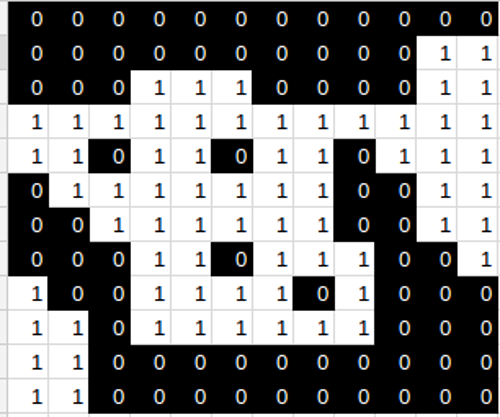
\includegraphics[scale=0.27]{pics/closing_o}
		\caption{Original Picture}
	\end{subfigure}
	\hfill
	\begin{subfigure}{.32\textwidth}
		\centering
		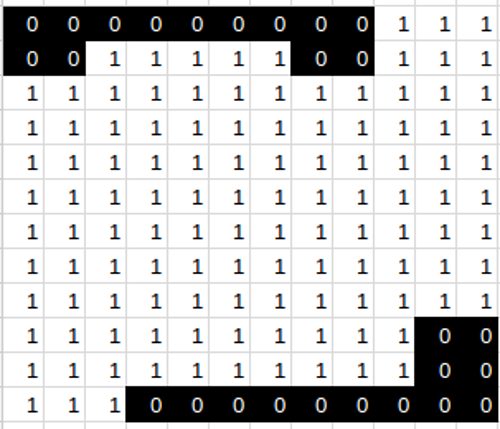
\includegraphics[scale=0.27]{pics/closing_d}
		\caption{Dilation stage}
	\end{subfigure}
	\hfill
	\begin{subfigure}{.32\textwidth}
		\centering
		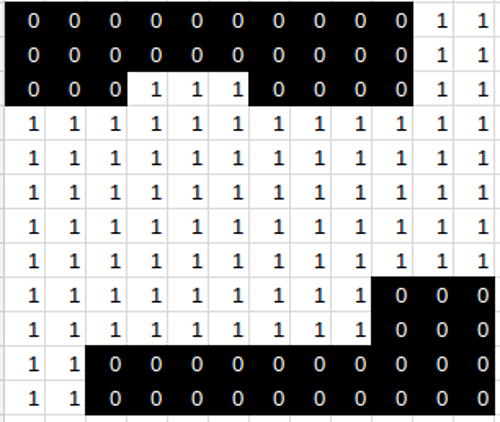
\includegraphics[scale=0.27]{pics/closing_e}
		\caption{Erosion stage}
	\end{subfigure}
	\caption{Closing operator step by step}
	\label{fig:closing}
\end{figure}



\subsubsection*{Image Registration}
% Lining up the AR to the paper
\subsubsection*{Feature Extraction}
% Possibly extracting known feature points like a house indicator

\subsubsection*{Image Differencing}
For users to be able to draw their own landscapes, there has to be some way
of recognising when there has been a change, physically, on paper. To 
automate this process will enable the program to decide for itself when
there has been an update to a drawing, rather than a user having to confirm each
time there is an update. Image differencing is the primary way of 
achieving this kind of detection. There are many different ways of actually
working out whether there is a "difference" between two images and some will
be further explained below. The general method for image differencing from
a video feed is taking two frames, at time $t_s$ and a time in the future
$t_{s+c}$ and compare the two.

\subsubsection*{Simple Intensity Differencing}
The simplest form of finding the difference between two images is comparing 
their pixel intensities. 
\begin{align}
	\begin{split}
		A \text{ is Image at time } t_{s} \\
		B \text{ is Image at time } t_{s+c} \\
		D \text{ is the difference Image } \\
		I(pixel) \text{ is the Intensity of the supplied pixel} \\
		\\
		D_{i,j} = | I(A_{i,j}) - I(B_{i,j}) | 	
	\end{split}
\end{align} 

Once the Difference Image has been computed, you can then perform a 
sum over all the pixels to get an indication into how much "change"
there was. Depending on if the image is grayscale, binary or RGB will
give different ranges of numbers, the higher the range, the less
this final sum will be able to tell you about the change in the image.
\\
A popular way to deal with this problem is to perform thresholding on
the Difference Image and is explained in Rosin's Paper
\textit{Thresholding for Change Detection}\cite{Rosin}. 
Again, there are different type of thresholding
such as Truncation, to-Zero, Binary and all of their inversions. 
For the purposes of this project, we will only look at Binary 
thresholding. \\

Binary thresholding takes a threshold value, $\tau$, which is 
acquired either through statistical or empirical methods. With
the threshold, any pixel value in the Difference Image that is below
the threshold is effectively ignored and set to 0. The pixels above
the threshold preserve their values. This method is very quick,
especially when considering grayscale images where the range of
pixel values is between the value 0 to 255. It begins a bit harder
to use Binary thresholding with images with more colour channels.

\begin{equation}
	D_{i,j} = 
	\begin{cases}
	0, & \text{ if $D_{i,j}$ $\leq$ $\tau$}. \\
	D_{i,j}, & \text{ otherwise}.
	\end{cases}
\end{equation}

By summing over these obtained values, the result may make more
sense as it is a representation of how many pixels in the image have
changed such that their change is significant. Of course this
"significance" is determined by the user and the chosen $\tau$.\\
\\
It is obvious that this is avery simple way of calculating difference
between images. To ensure accurate results, the camera has to stay
very still otherwise, potentially, every pixel could experience a 
change in intensity. This can be somewhwat countered by choosing
and appropriate $\tau$. However, if looking for finer changes, the
chosen $\tau$ could remove some of these changes, disabling detection.\\
\\
In addition, if the images are taken in different lighting environments
then that will cause inaccurate indications of difference. Take two
potential scenes, exactly the same and untouchedd camera fixed. In
the day time, the image captured will have a much higher intensity
than an image taken in the evening. This coud cause the whole image
to be above the threshold of changed but actually tell us nothing 
about changes in the scene, if any. The problem with dealing with
illumination changes becomes more prominent in surveillance literature.
A way to reduce the illumination effect is to perform a normalisation
of the pixels based on average intensities and variance. This shall
not be explained further but details of it and other detection 
techniques are highlighted it Radke's paper\cite{Radke04}.

\subsubsection*{Image Ratioing}
Image Ratioing is another method to compare images. The general concept
is explained (along with other change detection techniques) in Singh's
paper \textit{Review Article Digital change detection techniques 
using remotely-sensed data}\cite{Singh88}. Again we have our two images,
from before, taken at different times. From here, the pixels' intensities
are compared to obtain a ratio:

\begin{equation}
	R_{i,j} = \frac{A_{i,j}}{B_{i,j}}
\end{equation}

The closer this $R_{i,j}$ values is to 1, the more similar the two 
pixels are in terms of intensity. Thus, if $R_{i,j}$ is quite far from 
1, it is a good indicator that there has been change within the image.
Again, thresholding can be applied to ths Ratio Image, $R$, which will 
leave only those with a significant ratio to be considered. The same steps
as image differencing can then be utilised to gain a representation of the
overall change in the image.

\subsection*{Computer Graphics}

\subsubsection*{Camera alignment}

\subsection*{Existing Projects}

\subsubsection*{LandscapAR}
Looking into the Augmented reality scene and looking for potential similar
applications brought me across the mobile application \textit{LandscapAR},
made by Stapps. The premise of the application is that it is aimed at
graphic/landscape designers and turns drawn contour lines into an augmented
reality environment you can view through your phone screen. \\
\\
The application imposes several restrictions upon the user, however. The user
must use a thick black pen for the app to successfully identify contours. 
In addition, the user must make sure that every conour is properly connected
and closed. Already, this limits some things that the user is able to do, they
have to take the time to be precise and also must make sure they have the 
correct equipment to start creating their work. In addition, the application
requires the user to place white paper over a dark background/table otherwise
the scene may not be recognised. This is likely because they use the paper
edges as an anchor point upon which they can anchor the augmented data and 
use registration to align the output. \\
\\
There are several ways that this application can be improved. For example,
currently the user has to draw their contours on a piece of paper and then
scan paper using their mobile device. The scanning process itself is quite 
cumbersome as trying to get the system to detect paper can be hit and miss.
The scan analyses the image and overlays a 3D scene onto it quite well, however
the downfall with this is that to make updates to the scene, ou use has to
re-scan the image after addition, adding more cumbersome steps. For users
who want to make several small changes here and there, this will consume a lot
of time and effort on their part.
\\
\subsubsection*{The AR Sandbox}

%History
%What it can do

Nowadays, technology is obsessed with being more interactive, especially in 
the realm of games and education. With the emergence of hardware such as
Google Glass and the Oculus Rift, augmented and virtual reality is becoming
a hot and exciting field in which to make technological advances. Emphasis
has been made on "immersing ourselves" within the game or environment that
we are interacting with, in order to get a much more stimulating experience
which leaves a great impression upon us. I myself had taken a liking to 
Augmented Reality (AR) sometime before applying for my M.Eng Computing degree
at Imperial College London. This original interest provided most of the 
motivation for taking up this project.


\subsubsection*{Microsoft Kinect V2}
\underline{Background \& History}\\
The Microsoft Kinect(V1) was original released as an extra piece of hardware
for Microsoft's Xbox360 in 2010. The Kinect for windows (V2) was released
in 2012 and offered a range of improved statistics from its ancestor,
V1. Since its introduction into the market, the Kinect has received a lot of
attention from developers and there have been many applications for it put
forward\footnote{http://www.microsoft.com/en-us/kinectforwindows/meetkinect/gallery.aspx?searchv=entertainment}.
Many large companies have caught onto its capabilities and work 
alongside Microsoft and the Kinect.
\\ \\
In contrast to the Leap Motion, the Kinect V2 offers users the ability to track their 
whole body with reasonable accuracy. In addition, the V2 can track up to 6 individuals
at one time with 25 body joints able to be placed onto the captured images.
This opens up a whole new range of applications
that the Kinect can be used for and this is apparent in the amount of interest in the
Kinect, along with the amount of published papers and success stories of different
uses of it. Some of the possible fields this device can be used include 
Augmented Reality, Entertainment and Games, Retail, Education and much more. The 
Microsoft Kinect website highlights some of these interesting projects in more detail
\footnote{http://www.microsoft.com/en-us/kinectforwindows/meetkinect/default.aspx}.
\\ \\ 
The paper "Evaluation of the Spatial Resolution Accuracy of the Face 
tracking system for Kinect For Windows V1 and V2" \cite{AmonFuhrmann14}
explores in more detail the increase in performance and capability
of the V2 and shows that is beats V1 in every aspect. 
\\ \\
\underline{How it works} \\ 
The V2 allows us to take infrared images along with 1080p colour images. It 
also has depth sensors to produce depth images. Inside the V2 are 3 infrared
emitters along with a colour camera, an infrared camera and some microphones.
These internal components can be seen in figure \ref{kinectinternal}. The
microphones are along the bottom but will not be used within my project. 
\begin{center}
	\begin{figure}[H]
		\begin{center}
			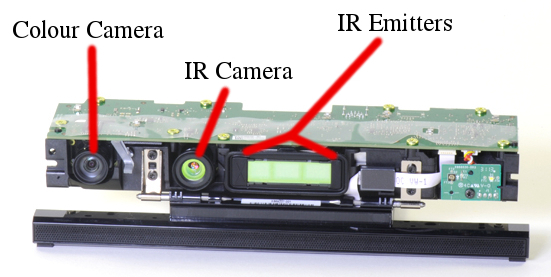
\includegraphics[scale=0.5]{pics/kinectinternal}
				\caption{Inside the Kinect V2 for Windows}
				\label{kinectinternal}
		\end{center}
	\end{figure}
\end{center}

The Kinect V2 differs from the V1 majorly in the way it produces depth maps.
V1 uses structured light while the V2 utilises Time-Of-Flight. Time-of-Flight
involves emitting many short bursts of infrared light (strobing it) and then
collecting it back through its camera. A very thorough discussion of how this
determines the depth of objects in the captured image is present on Daniel
Lau's blog \footnote{http://www.gamasutra.com/blogs/DanielLau/20131127/205820/The\_Science\_Behind\_Kinects\_or\_Kinect\_10\_versus\_20.php}.
The technique involves splitting a pixel in half and collecting infrared light
on the pixel. However, they are on at different times, while one half is on, 
the other is off and depending on the ratio of how much light is collected 
by each half (ratio since it accounts for light absorption by objects in the scene),
the relative depth of objects can be inferred. 
\\ \\
The V2 also accounts for over exposure and saturation of pixels. This scenario
occurs when there are alternative sources of infrared light, i.e. in an outdoor
environment! The V2 can reset pixel values in the middle of an exposure, also
explained in Daniel Lau's blog mentioned above. This then
allows it to be used outside where the V1 wouldn't account for this and cause
all kinds of strange behaviour; this of course means that the scope for using
the V2 and its applications is significantly larger than it ancestor.
\\ \\
\underline{My investigations} \\ \\
I investigated the Kinect for Windows first hand. In figure \ref{KinectDepth} 
you can see an example of the depth sensing capability of V2. On the right,
circled in blue, is myself. I sat around 40cm away from the camera. As I highlight 
in the limitations section below, this is reported as the minimum distance 
performance can be guaranteed by the V2. My friend, Juto Yu, is circled in 
yellow, he say slightly outside the view of the camera, giving me a rough 
indication on how wide the capture region is. The green circled object is a 
pillar in the central library of Imperial College, it is definitely more than 
3m away from the V2 which is reported as the range before objects become 
"too far". Whether it being detected is because the device can actually 
handle larger caption depths or due to the pillar being white and thus 
more reflective will need to be further looked in to.
\begin{center}
	\begin{figure}[H]
		\begin{center}
			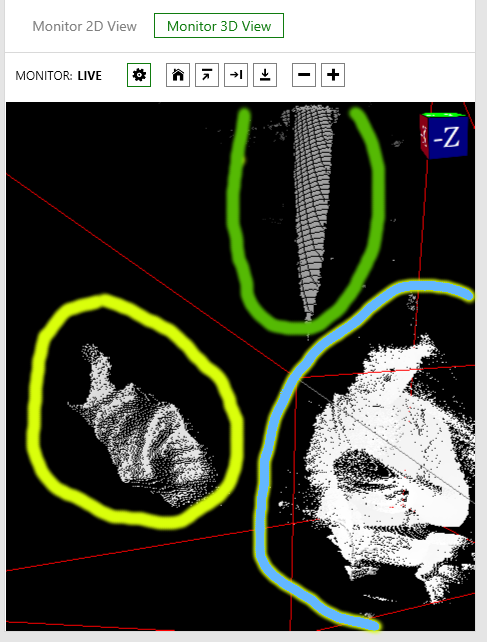
\includegraphics[scale=0.5]{pics/KinectDepth}
				\caption{Depth image from Kinect V2}
				\label{KinectDepth}
		\end{center}
	\end{figure}
\end{center}

I also looked into the colour camera's performance. The camera has a 1080p HD
video taking capability and is of a good quality. In addition, as seen in 
figure \ref{KinectColour}. The body tracking is pretty good and can make rather
accurate implications of people's limbs even when they are sitting down and are
obscured as shown. I was sitting at a desk but the V2 could make some guesses
as to where my legs would be. It is also clear that multiple tracking can be done
in real time at a speed that is responsive.
\begin{center}
	\begin{figure}[H]
		\begin{center}
			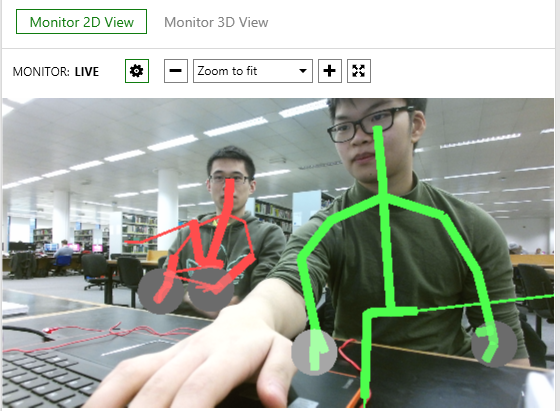
\includegraphics[scale=0.5]{pics/KinectColor}
				\caption{Colour Camera (with body tracking)}
				\label{KinectColour}
		\end{center}
	\end{figure}
\end{center}

The V2 is definitely a great alternative to some of the more expensive depth 
sensors on the market. As highlighted in the paper
"Low-cost commodity depth sensor comparison and accuracy analysis" by
Timo Breuer, Christoph Bodensteiner, Michael Arens. Some of the other sensors
that out perform it are upwards of £3000 while the V2 costs just around £150.
This means that it will be accessible to a much larger audience, something
definitely needed if an Augmented Reality game is to be successful.
\\ \\
\underline{Limitations and pitfalls}\\
The cameras of the V2 have a set range of values that it works well within.
This is reported by Microsoft to be from 0.4m to 3m
\footnote{https://msdn.microsoft.com/en-us/library/hh973078.aspx\#Depth\_Ranges}.
Anywhere beyond that seems to be too
far to determine the depth of objects. There is also a notion of being too near
to the device to! If we are working with the device, say, next to our laptop or
in a space nearby, there may be complications with how the sensor performs, 
anything closer than 0.4m produces unknown behaviour with the depth sensor.
\\ \\
A pitfall I expect to encounter is when developing with the Kinect SDK. I have
experience in C++ which is one of the languages that can be used to write Kinect 
applications. However, it seems a lot of the colour camera tutorials are written
in C\# which will could cause problems for me if I had to pick up the language 
or translate it into the C++ equivalents. However, this should only be a small
pitfall and cause minor hindrance to the progression of the project.

\newpage

\section*{Implementation}
In this section I will briefly outline the main steps I took to in
the creation of this project to tackle various problems.
\subsection*{Setting up the Camera and Environment}
\subsubsection*{Camera Calibration and Setup}
\subsubsection*{OpenCV}
\subsubsection*{OpenGL}
\subsection*{Capturing the Landscape map}
\subsubsection*{Drawing the map}
\subsubsection*{Detecting Contours}
\subsubsection*{Genearting the Hierarchy Tree}
\subsection*{Generating the 3D scene}
\subsubsection*{View Point alignment}
\subsubsection*{Using the Hierarchy Tree}
\subsubsection*{Terrain Generation}
\subsection*{Detecting change in the scene}
\subsubsection*{Generating the Base image}
\subsubsection*{Introducting change}
\subsubsection*{Determining Stabilisation}
\subsection*{Restructure and regenerating the 3D scene}
\subsubsection*{Generating a Difference Image}
\subsubsection*{Determining new contours}
\subsubsection*{Updating the the Hierarchy Tree}
\subsubsection*{Adding in the environment change}

\section*{Evaluation}
\subsection*{Test Measures}
\subsection*{Indicators of Success}
\subsection*{User Testing}
\subsubsection*{Responsiveness}
\subsubsection*{Aesthetics}
\subsection*{Results}
\subsection*{Overall Evaluation}

\section*{Extensions}
Having implemented an environment for dynamic creative Augmented Reality,
content, there are many obvious improvements that can be made to transform 
this project into a much larger and better application. \\
\\
The original idea for this project was the concept of having an environment
for individuals to create their own 3D, responsive landscapes that can react
to changes in the real world scene and reflect them within the AR scene. Indeed
this has been done to a certain extent, changes in the landscape drawing cause
the AR scene to change as a result, without need for user interaction with the
program. Currently this only works with contour to landscape conversion. This
will be of little use to individuals who wish to create something more than just
land. In this section shall highlight some of the more immediate extensions
and then go on to explore other extensions which have been lingering in the 
background of my vision for what this project could have become.

\subsection*{Immediate Extensions}
There are numerous extensions that can be added to this project due to the 
vast amounts of things that could be brought to life by Augmented Reality.
These are the extensions I would have implemented had I more time to commit
to this project.

\subsubsection*{Coloured Contours}
Currently the program works by taking frames from the camera and then   
processing them with various operations, such as perform morphological
closing and blurring by the Canny Edge detector. One additional thing 
which can be done is to allow and detect coloured contours. Right now,
if three sets of contours drawn in different colours were presented to
the program, they would all behave the same way and create a terrain
with a green shade. If we were to introduce new colours, we could also
introduce new terrain! For example, brown tinted colours could represent
rock or mountainous landscape; green can be used to represent something like
everything within is a cluster of trees i.e. a forest! Blue can signify
the enclosed area is a lake or a body of water. The things different
colours can represent are endless and will add an extra amount of creativity
(and enjoyment) to the application! One use for this is creating a 
landscape for a battlefield or any other kind of more detailed environments.
These in turn can be used to protoype landscapes for games!\\
\\
To implement this wouldn't require much extension to the program. Just a simple
reading of the contour points' RGB values and from there making a distance 
measure which will allow classification of the considered pixels to the 
closest colour. From there, generation of the 3D scene will be a switch case 
between different terrains base on the result of the classification.

\subsubsection*{Other markers}
A marker is something on the paper or creative environment that will be 
detected and understood by the program. Right now, the only markers we have
at the user's disposal are contour lines which are converted into land with
different elevation levels. While it is very easy to add special computer
generated markers
 						it removes from the creative experience of the application
as there is less interaction with pen and paper. \\
\\
To have other markers which represent other objects would greatly enhance the
creative power of the user. Some examples of these are converting crosses ("X")
into trees, drawn stars into houses or buildings, we can even add in animals 
or people with more markers and have them traverse the scene. Other than this
last point, the other marker ideas require little extra logic to implement.
By having a lookup table of shapes used as markers and what they represent, we
can easily perform a template matching algorithm. OpenCV offers a matching
algorithm which compares two images. We can extract markers drawn onto the
surface and compare them against stored markers by passing the stored marker
over the image as some kind of mask for convolution. A difference measure is run
across the two images (taking into account rotation and affine transformation).
If this is smaller than a threshold then it can be said within some statiscal
region, that the detected area was intended to be that marker. From there placing
the object over the mid point (with regard to surface normal) will suffice.

\subsubsection*{Photorealistic lighting environment}
Augmented Reality comes under the fields of Computer Graphics and Computer
Vision, and as a result it means that for it to be good, it has to look good.
The potential user of this program can range from professional land/environment
planner all the way to a 3 year old child with a bunch of pens at their 
disposal. If it does not appealing, it will not appeal to the professional
and the sustained interest of the 3 year old cannot be guaranteed by 
sub-standard graphics. A very easy way to quickly improve a scene and make it
realistic, as Augmented Reality should be, is to add illumination equivalent 
to the local scene. \\
\\
Implementing this also shouldn't require too much extra logic and is something
I wanted to be able to add into the project; unfortunately I had not
enough time due to unexpected road blocks within other areas of the project.
By using a light probe placed within view of the camera, global illumination
can be achieved without much intereference to the scene. A single frame can be
enough to get the lighting for the environment. In addition, this can change 
with time as the environment can be update every so often wither by frame count
or program run time, where another frame will be taken and the environment 
recalculated in the background. As a result, when lighting conditions change
over time, it will cause no problem to the user and require no extra interaction.\\
\\
Another point to think about is shadowing and self occlusion which should 
cause shadows to form upon the landscape creataed by other parts of the landscape
itself. This would be included once the global illumination has been captured.

\subsection*{Future Extensions}
I shall now highlight some of the other ideas I had while going into this 
project although some were a bit too broad and not realted enough to the main
goals and contributions of this project. These extensions are more of what
can be done to grow this project into a fully functions piece of software that
could potnetially be used commercially, or indeed lay groundwork for future
work in Augmented Reality. There are also ideas here that could be implemented
when the technology for its realisation becomes available.

\subsubsection*{The Leap Motion}
Before coming into this project I had a great interest and desire to work with
some of the newer technologies such as touchless controls, Virtual Reality 
head pieces and Augmented Reality. While investigating these, I ran into the
Leap Motion, an infrared hand tracker which allows you to use your hands as
an input device. I really loved the idea of using your own hands to interact
with things in a generated environment as opposed to touchless control of a device.
However, the leap motion still has a number of bugs and is not as seamless and 
hand tracking as one would like it to be. It is still one of the better and 
cheaper hand tracking devices out there, with advances in its development I think
it could prove very useful to users of the AR program created from this project.\\
\\
The basic idea for integrating this piece of hardware into the project is to,
after creating the scene, the user is also able to \textit{manipulate} the
scene they had just created! This adds another dimension onto the creative
ability of the the application and really promotes the basic idea I have when
conducting this project. Using your hands to create things! \\
\\
On top of this basic idea, there were a variety of potential pieces of 
functionality that could be implemented with this new medium of interaction, some
of which I shall list:

\begin{enumerate}
	\item \textit{Allow the user to scale the environment using their hands.} \\
		  By registering a pinch action, if the user pinches edges of the
		  generated scene, or by pinching the highest point and pulling 
		  outward/upward, the user can scale the generated scene to their 
		  desired size! Will require alignment of Leap Motion hand point 
		  coordinate space to the 3D scene coordinate space to work.
	\item \textit{Adding content by drag and drop.}
		  This functionality is inspired by games much like \textit{The Sims}.
		  The user can choose to either add in content through the computer and
		  literally drop it into the scene by moving their hands around. This
		  could possibly be achieves by pinch and release as aforementioned. 
		  If the extension of adding in animals/people or other moving object
		  that traverse the scene were to implemented, the user could also
		  pick these up and move them around the scene at will. This will 
		  introduce more of a game aspect into the project and will definitely
		  appeal to the younger set of users while adding functionality for
		  those who could be using this for professional work.
	\item \textit{Introduce "God Mode"}
		  Again inspired by some games and similar to the above point. Allow
		  the user to view hands in the scene, as if you were playing the
		  role of God. This is purely to enchance the program as more of a game
		  instead of a creative environment. God mode would allow the user to
		  make various changes to the environment, for example spreading the hand
		  could represent rainfall on the area below the convex hull of the hand
		  points! Another idea is if the user start  pressing on the landscape, the
		  landscape itself can change, e.g. decreasing in height, cause cracks in
		  the scene etc. This is one of the more ambitious extensions.
\end{enumerate}

\subsubsection*{No Calibration Marker}


\subsubsection*{Continued testing and experimentation} 
Some shit here \\
\\
\\
\\

\newpage

\bibliographystyle{plain}
\bibliography{biblio}
\end{document}
